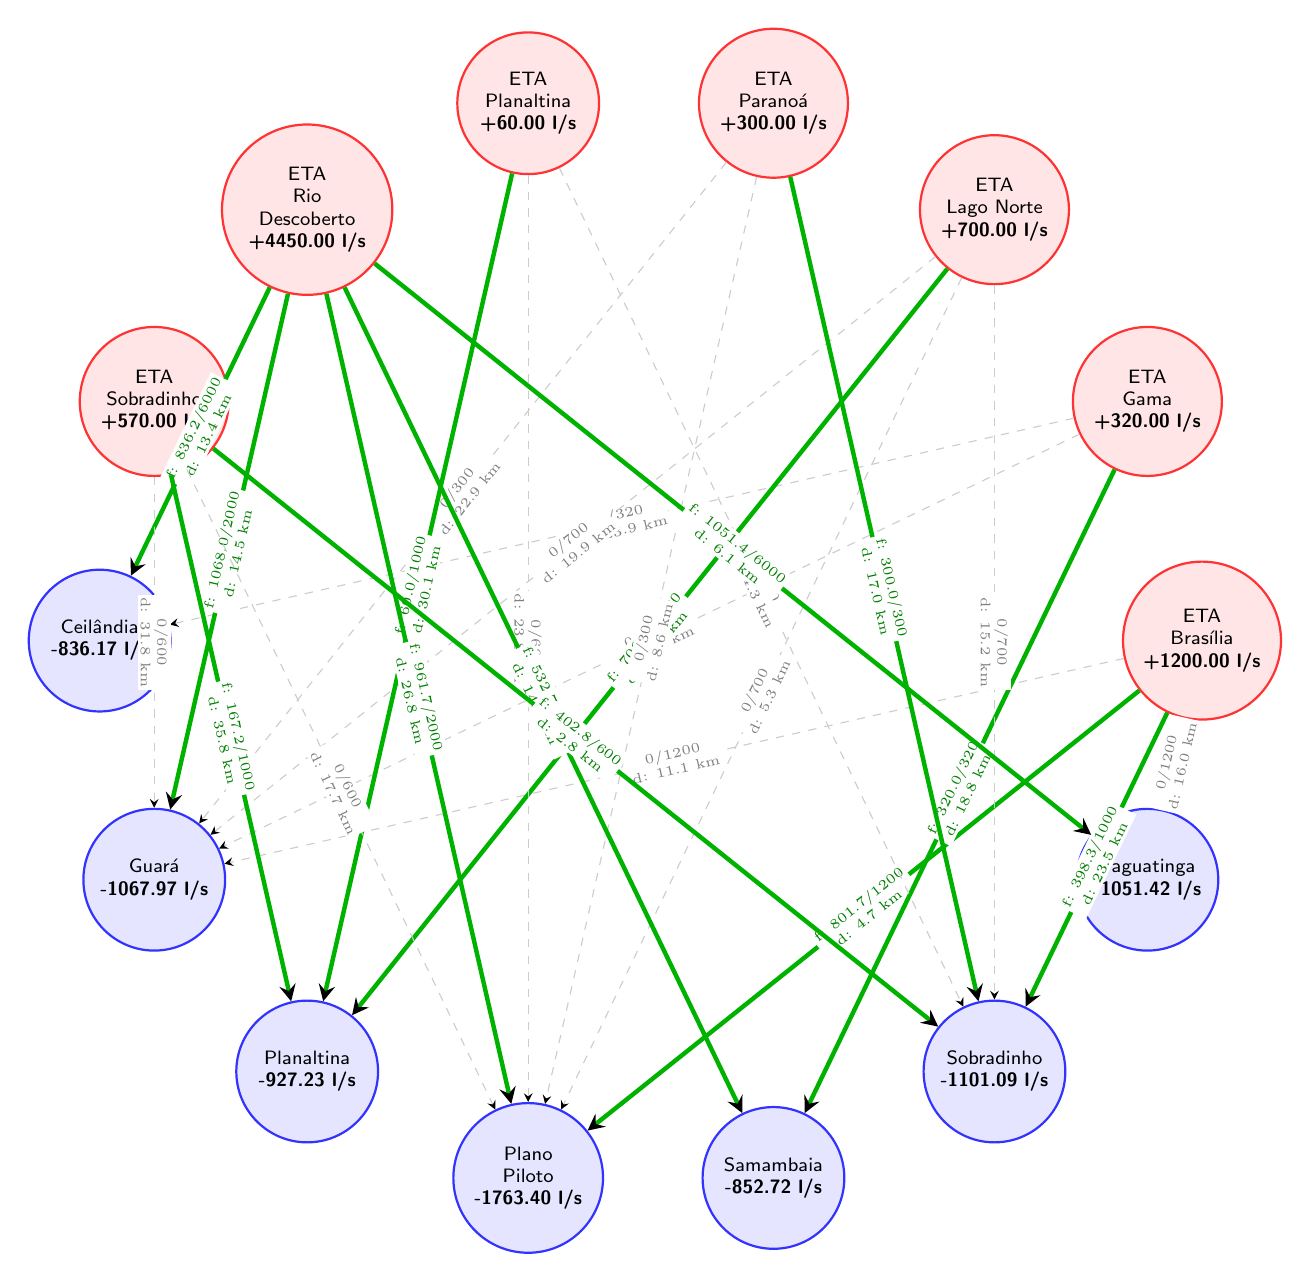
\begin{tikzpicture}[>=stealth, node distance=4.5cm, every node/.style={font=\sffamily\scriptsize}]
  \tikzstyle{eta}=[circle, draw=red!80, fill=red!10, thick, minimum size=1.8cm, align=center]
  \tikzstyle{ra}=[circle, draw=blue!80, fill=blue!10, thick, minimum size=1.8cm, align=center]
  \tikzstyle{active_edge}=[draw=green!70!black, ->, ultra thick]
  \tikzstyle{inactive_edge}=[draw=gray!40, ->, dashed, thin]

  % Node positions
  \node[eta] (eta_brasilia) at (0.0:7.00) {ETA\\ Brasília\\ \textbf{+1200.00 l/s}};
  \node[eta] (eta_gama) at (25.714285714285715:7.00) {ETA\\ Gama\\ \textbf{+320.00 l/s}};
  \node[eta] (eta_lago_norte) at (51.42857142857143:7.00) {ETA\\ Lago Norte\\ \textbf{+700.00 l/s}};
  \node[eta] (eta_paranoa) at (77.14285714285714:7.00) {ETA\\ Paranoá\\ \textbf{+300.00 l/s}};
  \node[eta] (eta_planaltina) at (102.85714285714286:7.00) {ETA\\ Planaltina\\ \textbf{+60.00 l/s}};
  \node[eta] (eta_rio_descoberto) at (128.57142857142858:7.00) {ETA\\ Rio\\ Descoberto\\ \textbf{+4450.00 l/s}};
  \node[eta] (eta_sobradinho) at (154.28571428571428:7.00) {ETA\\ Sobradinho\\ \textbf{+570.00 l/s}};
  \node[ra] (ceilândia) at (180.0:7.00) {Ceilândia\\ \textbf{-836.17 l/s}};
  \node[ra] (guara) at (205.71428571428572:7.00) {Guará\\ \textbf{-1067.97 l/s}};
  \node[ra] (planaltina) at (231.42857142857142:7.00) {Planaltina\\ \textbf{-927.23 l/s}};
  \node[ra] (plano_piloto) at (257.14285714285717:7.00) {Plano\\ Piloto\\ \textbf{-1763.40 l/s}};
  \node[ra] (samambaia) at (282.85714285714283:7.00) {Samambaia\\ \textbf{-852.72 l/s}};
  \node[ra] (sobradinho) at (308.57142857142856:7.00) {Sobradinho\\ \textbf{-1101.09 l/s}};
  \node[ra] (taguatinga) at (334.2857142857143:7.00) {Taguatinga\\ \textbf{-1051.42 l/s}};

  % Pipe connections
  \path[active_edge] (eta_brasilia) edge node[draw=none,fill=white,inner sep=1pt,sloped,align=center,font=\tiny\color{green!50!black}] {f: 801.7/1200\\ d: 4.7 km} (plano_piloto);
  \path[inactive_edge] (eta_brasilia) edge node[draw=none,fill=white,inner sep=1pt,sloped,align=center,font=\tiny\color{gray}] {0/1200\\ d: 11.1 km} (guara);
  \path[inactive_edge] (eta_brasilia) edge node[draw=none,fill=white,inner sep=1pt,sloped,align=center,font=\tiny\color{gray}] {0/1200\\ d: 16.0 km} (taguatinga);
  \path[active_edge] (eta_brasilia) edge node[draw=none,fill=white,inner sep=1pt,sloped,align=center,font=\tiny\color{green!50!black}] {f: 398.3/1000\\ d: 23.5 km} (sobradinho);
  \path[active_edge] (eta_gama) edge node[draw=none,fill=white,inner sep=1pt,sloped,align=center,font=\tiny\color{green!50!black}] {f: 320.0/320\\ d: 18.8 km} (samambaia);
  \path[inactive_edge] (eta_gama) edge node[draw=none,fill=white,inner sep=1pt,sloped,align=center,font=\tiny\color{gray}] {0/320\\ d: 20.3 km} (guara);
  \path[inactive_edge] (eta_gama) edge node[draw=none,fill=white,inner sep=1pt,sloped,align=center,font=\tiny\color{gray}] {0/320\\ d: 23.9 km} (ceilândia);
  \path[inactive_edge] (eta_lago_norte) edge node[draw=none,fill=white,inner sep=1pt,sloped,align=center,font=\tiny\color{gray}] {0/700\\ d: 5.3 km} (plano_piloto);
  \path[inactive_edge] (eta_lago_norte) edge node[draw=none,fill=white,inner sep=1pt,sloped,align=center,font=\tiny\color{gray}] {0/700\\ d: 15.2 km} (sobradinho);
  \path[inactive_edge] (eta_lago_norte) edge node[draw=none,fill=white,inner sep=1pt,sloped,align=center,font=\tiny\color{gray}] {0/700\\ d: 19.9 km} (guara);
  \path[active_edge] (eta_lago_norte) edge node[draw=none,fill=white,inner sep=1pt,sloped,align=center,font=\tiny\color{green!50!black}] {f: 700.0/1000\\ d: 42.8 km} (planaltina);
  \path[inactive_edge] (eta_paranoa) edge node[draw=none,fill=white,inner sep=1pt,sloped,align=center,font=\tiny\color{gray}] {0/300\\ d: 8.6 km} (plano_piloto);
  \path[active_edge] (eta_paranoa) edge node[draw=none,fill=white,inner sep=1pt,sloped,align=center,font=\tiny\color{green!50!black}] {f: 300.0/300\\ d: 17.0 km} (sobradinho);
  \path[inactive_edge] (eta_paranoa) edge node[draw=none,fill=white,inner sep=1pt,sloped,align=center,font=\tiny\color{gray}] {0/300\\ d: 22.9 km} (guara);
  \path[inactive_edge] (eta_planaltina) edge node[draw=none,fill=white,inner sep=1pt,sloped,align=center,font=\tiny\color{gray}] {0/60\\ d: 4.3 km} (sobradinho);
  \path[inactive_edge] (eta_planaltina) edge node[draw=none,fill=white,inner sep=1pt,sloped,align=center,font=\tiny\color{gray}] {0/60\\ d: 23.8 km} (plano_piloto);
  \path[active_edge] (eta_planaltina) edge node[draw=none,fill=white,inner sep=1pt,sloped,align=center,font=\tiny\color{green!50!black}] {f: 60.0/1000\\ d: 30.1 km} (planaltina);
  \path[active_edge] (eta_rio_descoberto) edge node[draw=none,fill=white,inner sep=1pt,sloped,align=center,font=\tiny\color{green!50!black}] {f: 1051.4/6000\\ d: 6.1 km} (taguatinga);
  \path[active_edge] (eta_rio_descoberto) edge node[draw=none,fill=white,inner sep=1pt,sloped,align=center,font=\tiny\color{green!50!black}] {f: 836.2/6000\\ d: 13.4 km} (ceilândia);
  \path[active_edge] (eta_rio_descoberto) edge node[draw=none,fill=white,inner sep=1pt,sloped,align=center,font=\tiny\color{green!50!black}] {f: 532.7/6000\\ d: 14.2 km} (samambaia);
  \path[active_edge] (eta_rio_descoberto) edge node[draw=none,fill=white,inner sep=1pt,sloped,align=center,font=\tiny\color{green!50!black}] {f: 1068.0/2000\\ d: 14.5 km} (guara);
  \path[active_edge] (eta_rio_descoberto) edge node[draw=none,fill=white,inner sep=1pt,sloped,align=center,font=\tiny\color{green!50!black}] {f: 961.7/2000\\ d: 26.8 km} (plano_piloto);
  \path[active_edge] (eta_sobradinho) edge node[draw=none,fill=white,inner sep=1pt,sloped,align=center,font=\tiny\color{green!50!black}] {f: 402.8/600\\ d: 2.8 km} (sobradinho);
  \path[inactive_edge] (eta_sobradinho) edge node[draw=none,fill=white,inner sep=1pt,sloped,align=center,font=\tiny\color{gray}] {0/600\\ d: 17.7 km} (plano_piloto);
  \path[inactive_edge] (eta_sobradinho) edge node[draw=none,fill=white,inner sep=1pt,sloped,align=center,font=\tiny\color{gray}] {0/600\\ d: 31.8 km} (guara);
  \path[active_edge] (eta_sobradinho) edge node[draw=none,fill=white,inner sep=1pt,sloped,align=center,font=\tiny\color{green!50!black}] {f: 167.2/1000\\ d: 35.8 km} (planaltina);
\end{tikzpicture}